\documentclass[11pt,a4paper]{article}

% für \hyphenation mit Umlauten
\usepackage[T1]{fontenc}
\usepackage[utf8]{inputenc}
\usepackage[ngerman,english]{babel}

% Times-Roman-Schrift (auch für mathematische Formeln)
\usepackage{mathptmx} 

% comments
\usepackage{verbatim} 

% Zum Setzen von URLs
\usepackage{color}
\usepackage{alltt}
\definecolor{darkred}{rgb}{.25,0,0}
\definecolor{darkgreen}{rgb}{0,.2,0}
\definecolor{darkmagenta}{rgb}{.2,0,.2}
\definecolor{darkcyan}{rgb}{0,.15,.15}
\definecolor{LightButter}{rgb}{0.98,0.91,0.31}
\definecolor{LightOrange}{rgb}{0.98,0.68,0.24}
\definecolor{LightChocolate}{rgb}{0.91,0.72,0.43}
\definecolor{LightChameleon}{rgb}{0.54,0.88,0.20}
\definecolor{LightSkyBlue}{rgb}{0.45,0.62,0.81}
\definecolor{LightPlum}{rgb}{0.68,0.50,0.66}
\definecolor{LightScarletRed}{rgb}{0.93,0.16,0.16}
\definecolor{Butter}{rgb}{0.93,0.86,0.25}
\definecolor{Orange}{rgb}{0.96,0.47,0.00}
\definecolor{Chocolate}{rgb}{0.75,0.49,0.07}
\definecolor{Chameleon}{rgb}{0.45,0.82,0.09}
\definecolor{SkyBlue}{rgb}{0.20,0.39,0.64}
\definecolor{Plum}{rgb}{0.46,0.31,0.48}
\definecolor{ScarletRed}{rgb}{0.80,0.00,0.00}
\definecolor{DarkButter}{rgb}{0.77,0.62,0.00}
\definecolor{DarkOrange}{rgb}{0.80,0.36,0.00}
\definecolor{DarkChocolate}{rgb}{0.56,0.35,0.01}
\definecolor{DarkChameleon}{rgb}{0.30,0.60,0.02}
\definecolor{DarkSkyBlue}{rgb}{0.12,0.29,0.53}
\definecolor{DarkPlum}{rgb}{0.36,0.21,0.40}
\definecolor{DarkScarletRed}{rgb}{0.64,0.00,0.00}
\definecolor{Aluminium1}{rgb}{0.93,0.93,0.92}
\definecolor{Aluminium2}{rgb}{0.82,0.84,0.81}
\definecolor{Aluminium3}{rgb}{0.73,0.74,0.71}
\definecolor{Aluminium4}{rgb}{0.53,0.54,0.52}
\definecolor{Aluminium5}{rgb}{0.33,0.34,0.32}
\definecolor{Aluminium6}{rgb}{0.18,0.20,0.21}

\usepackage[plainpages=false,bookmarks=true,bookmarksopen=true,colorlinks=true,
  linkcolor=darkred,citecolor=darkgreen,filecolor=darkmagenta,
  menucolor=darkred,urlcolor=darkcyan]{hyperref}

% Zeilenabstand
\renewcommand{\baselinestretch}{1.5}

% anhang
\usepackage[toc,page]{appendix}

% pdflatex: Bilder in den Formaten .jpeg, .png und .pdf
% latex: Bilder im .eps-Format
\usepackage{graphicx}

\usepackage{fancyhdr} % Positionierung der Seitenzahlen
\fancyhead[R]{}
\fancyfoot[R]{\Roman{page}}

\renewcommand{\headrulewidth}{0pt}

 % behebt headheight Warning
\setlength{\headheight}{13.6pt}

% Korrektes Format für Nummerierung von Abbildungen (figure) und
% Tabellen (table): <Kapitelnummer>.<Abbildungsnummer>
\makeatletter
\@addtoreset{figure}{section}
\renewcommand{\thefigure}{\thesection.\arabic{figure}}
\@addtoreset{table}{section}
\renewcommand{\thetable}{\thesection.\arabic{table}}
\makeatother

% Listings für Sourcecode
\usepackage{listings}
  \usepackage{courier}
 \lstset{
        basicstyle=\footnotesize\ttfamily, % Standardschrift
        numbers=left,               % Ort der Zeilennummern
        numberstyle=\tiny,          % Stil der Zeilennummern
        %stepnumber=2,               % Abstand zwischen den Zeilennummern
        numbersep=5pt,              % Abstand der Nummern zum Text
        tabsize=2,                  % Groesse von Tabs
        extendedchars=true,         %
        breaklines=true,            % Zeilen werden Umgebrochen
        keywordstyle=\color{red},
        frame=b,         
        keywordstyle=[1]{\color{DarkSkyBlue}},    % Stil der Keywords
        keywordstyle=[2]{\color{DarkScarletRed}},    %
        keywordstyle=[3]{\bfseries},    %
        keywordstyle=[4]{\color{DarkPlum}},    %
        keywordstyle=[5]{\color{SkyBlue}},    %
		stringstyle={\color{Chocolate}},
        showspaces=false,           % Leerzeichen anzeigen ?
        showtabs=false,             % Tabs anzeigen ?
        xleftmargin=17pt,
        framexleftmargin=17pt,
        framexrightmargin=5pt,
        framexbottommargin=4pt,
        backgroundcolor=\color{Aluminium1},
        showstringspaces=false,      % Leerzeichen in Strings anzeigen ?
		%language=php
		morekeywords=[1]{Interface,return,static,function}
}
    %\DeclareCaptionFont{blue}{\color{blue}} 

  %\captionsetup[lstlisting]{singlelinecheck=false, labelfont={blue}, textfont={blue}}
  \usepackage{caption}
\DeclareCaptionFont{white}{\color{white}}
\DeclareCaptionFormat{listing}{\colorbox[cmyk]{0.43, 0.35, 0.35,0.01}{\parbox{\textwidth}{\hspace{15pt}#1#2#3}}}
\captionsetup[lstlisting]{format=listing,labelfont=white,textfont=white, singlelinecheck=false, margin=0pt, font={bf,footnotesize}}
\renewcommand\lstlistingname{Codeblock}
 

\sloppy % Damit LaTeX nicht so viel über "overfull hbox" u.Ä. meckert

% Ränder
\addtolength{\topmargin}{-16mm}
\setlength{\oddsidemargin}{40mm}
\setlength{\evensidemargin}{40mm}
\addtolength{\oddsidemargin}{-1in}
\addtolength{\evensidemargin}{-1in}
\setlength{\textwidth}{13cm}
\addtolength{\textheight}{34mm}
%______________________________________________________________________

\hypersetup{
	pdfauthor = {Franziskus Domig, Stefan Gassner, BSc; BSc; Wolfgang Halbeisen, BSc; Matthias Schmid, BSc},
	pdftitle = {Projekt Dokumentation Roadrunner},
	pdfkeywords = {Roadrunner, Dokumentation, Transport, Logistik},
}

%======================================================================
%
%      Document
%
%======================================================================

\begin{document}

\selectlanguage{ngerman}

\pagestyle{empty} % Vorerst keine Seitenzahlen
\pagenumbering{alph} % Unsichtbare alphabetische Nummerierung

\begin{center}
\textsc{Fachhochschule Vorarlberg GmbH}\\

\vspace{5cm}
{\large\textbf{Projekt Dokumentation}}\vspace{.5cm}

{\LARGE Roadrunner}

\vspace{10cm}
ausgeführt von\\
{\large
Franziskus Domig, Bsc;\\
Stefan Gassner, BSc;\\
Wolfgang Halbeisen, BSc;\\
Matthias Schmid, BSc}\\
\vfill

\end{center}

\begin{tabular}{ll}
Bearbeitung: & Dornbirn, im Frühjahr 2011\\
Betreuer: & XXX\\
\end{tabular}
%______________________________________________________________________


\section{Vorwort}

TODO

\clearpage
\section{Spezifikation}
\label{sec:specification}

Roadrunner ist ein System zur Überwachung von Arzneimittel-Transporten. Es verwaltet Waren in einem Backend-System, welches ein verteiltes Datenbanksystem verwendet. Mit mobilen Android-Geräten wird der Transport sowie die Lagerung von Zustellern sowie Lagermitarbeitern überwacht.

Transport von medizinischen Produkten (temperatursensitiv, Transportzeit, überwachbar, etc.).

\subsection{Technologie}

\begin{itemize}
	\item Backend-/Application-Server
	\item Annahmestelle für Waren (Item)
	\item verteilte Datenbank (CouchDB)
	\item Android für mobile Überwachung der Sensoren/Position/etc.
	\item Sensoren
		\begin{itemize}
			\item WLAN: Zugriff mit bspw. \verb=http://192.168.47.11:1234/=
			\item Bluetooth: TODO Matze
		\end{itemize}
	\item Barcode-Lesegerät mit Android Devices
		\begin{itemize}
			\item Barcode-Scanner App\\
			\verb=Activity.forResult (com.google.zxing.client.android.SCAN);=
		\end{itemize}
\end{itemize}

\subsection{Fragestellungen}

CouchDB für diese Anwendung sinnvoll, machbar? Ja.

Barcode mit Android-Device lesbar? Schnell genug? Ist ein Framework verfügbar?

Sensoren mit Bluetooth auslesbar? PAN? Alternativen (evt. WLAN/HTTP)?



\clearpage
\section{Technologie}
\label{sec:technology}

In diesem Abschnitt werden die von diesem Projekt verwendeten Technologien erläutert. Insbesondere werden die Gründe beschrieben, weswegen diese Technologien eingesetzt und anderen vorgezogen werden. Die Vor- sowie Nachteile der entsprechenden Technologien werden gegenübergestellt und besprochen. Zugleich werden die entsprechenden Technologien auf ihre Tauglichkeit in einem real logistischen Szenario geprüft.

\subsection{CouchDB}
\label{subsec:couchdb}
CouchDB\footnote{The Apache CouchDB Project, \url{http://couchdb.apache.org/}} ist eine auf die Verwaltung von Dokumenten basierte Datenbank. CouchDB kann ähnlich wie das MapReduce Framework von Google\footnote{vgl. \url{http://en.wikipedia.org/wiki/MapReduce}} abgefragt sowie indiziert werden.

TODO: Ausführlicher beschreiben.

\subsection{Node.js}
\label{subsec:nodejs}

Node.js ist ein ereignisgesteuertes I/O Framework für die V8 JavaScript Engine \cite{Wikipedia10a}. Diese wurde in C++ sowie JavaScript entwickelt und liegt in einer MIT-Lizenz vor, welches es für dieses Projekt einsetzbar macht und zugleich auch in einem realen Szenario eingesetzt werden könnte.

Mit Node.js können mit wenigen Zeilen Code, Server-Applikationen programmiert werden. Es wird hierzu auf einem Interface (IP) sowie einem beliebigen Port eine JavaScript Callback-Funktion registriert, welche bei einem Zugriff aufgerufen wird. Dies macht es sehr einfach, Sensoren in diesem System zu simulieren, welche via HTTP-Requests ``ausgelesen'' werden können.


\subsection{PHP - Silex}

PHP ist eine dynamische Skriptsprache, die speziell für den Einsatz auf Webservern entwickelt wurde. Jegliche Anfrage an eine PHP-Datei auf einem entsprechend konfigurierten Webserver wird durch die \emph{PHP-Runtime} interpretiert. Dabei wird eine passende Antwort generiert und durch den Webserver an den Client gesendet. Dies stellt die Basis für eine dynamische Webseite mit PHP dar. PHP ist verfügbar für eine breite Anzahl an Webservern, sowie für unterschiedlichste Plattformen wie Linux, Mac OS X, Windows oder Unix.

Silex\footnote{vgl. \url{http://silex-project.org}} ist ein Mikroframework für PHP 5.3. Es basiert wiederum auf dem Kern des Symfony2\footnote{vgl. \url{http://symfony.com}} Framework.

\subsection{Android/Java}

TODO

\subsection{Barscanner}

TODO

\clearpage
\section{Usecases}


\begin{itemize}
  \item Wareneingang
  	\subitem registriert Pakete im System
  	\subitem klebt QR-Code auf Pakete

	\item Logister plant und erstellt Lieferungen (neue Auftragsnummer wird
	generiert) \subitem wählt Pakete aus (können mit Sensoren bestückt sein)
		\subitem wählt Fahrer aus 
		\subitem wählt Transportmittel (können mit Sensoren bestückt sein) für
		Lieferungen aus
		\subitem trägt Zielort und Auftraggeber ein
  	
  \item Transporteur
  	\subitem holt oder hat Device mit Roadrunner App
  	\subitem loggt sich im Roadrunner System ein
  		\subsubitem mit Benutzerdaten wird sein/e aktuelle/r Auftrag/Lieferung aufs
  		Device synchronisiert ODER 
  		\subsubitem scannt Pakete und lädt sie in das vom Logistiker ausgwählte
  		Transportmittel
\end{itemize}

\paragraph{Daten-Synchronisierung}
	\textbf{Vorbedingungen: }
	\begin{itemize}
	  \item Transporteur hat sich in der System-App eingeloggt
	\end{itemize}
	
	Die Daten-Synchronisierung oder Replizierung wird durch das Einloggen im
	System angestoßen. Das mobile Gerät erhält folgende Information:
	\begin{itemize}
	  \item Adressen der Sensoren, die das Gerät überwachen sollte
	  \item alle Produkte, Pakete der aktuellen Lieferung, sowie Zielort, etc.
	  \item Überwachungs-Thresholds der Pakete
	\end{itemize}
\par


\clearpage
\section{Iteration 1}

\subsection{Ziele}

\begin{itemize}
  \item Produkte können erzeugt werden.
  \item Produkte können eingelagert werden.
  \item Produkte können ausgelagert werden.
\end{itemize}

\subsection{UML}

\begin{figure}
	\centering
		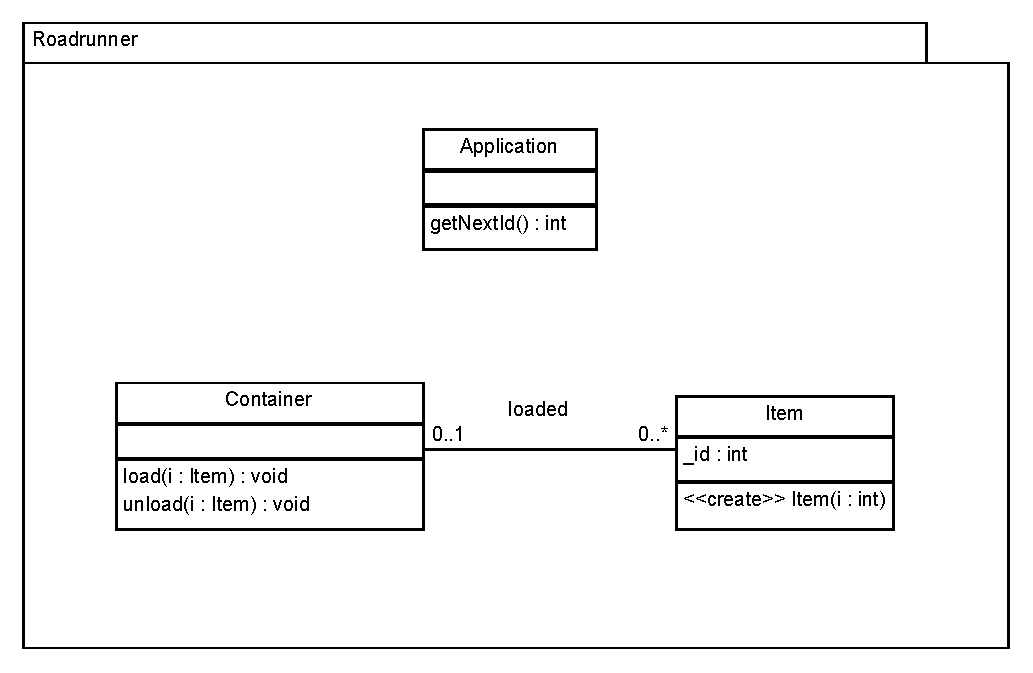
\includegraphics[width=\textwidth]{files/pdf/Iteration1.pdf}
	\caption{Iteration 1}
	\label{fig:Iteration1}
\end{figure}


\clearpage
\section{Sicherheit}

\subsection{Zeitsynchronisierung}

In diesem Abschnitt werden Probleme besprochen, die durch fehlerhafte respektive
mangelhaft durchdachte Zeitsynchronisierung oder Verbindungsabbruch entstehen
können.


\paragraph{Problem durch falsche Zeitstempel bei Logeinträgen:}
Betrachtet wird das Szenario ``Umladevorgang eines Produktes''. Das mobile
Gerät der Transporteinheit wird benutzt um den Ausladevorgang aus einem
Container im System zu verarbeiten. Mit dem scannen des Produkts wird auf dem
mobilen Gerät der Transporteinheit ein Logeintrag in dessen lokale Datenbank
erstellt. Genauso wird beim darauffolgenden Ladevorgang der Umladestation ein
Logeintrag auf dessen Gerät erstellt. Wenn das System mit absoluter Zeit
arbeitet und die Uhrzeit des Geräts der Transporteinheit vor jener der
Umladestation ist, dann würde im System der Übernahmevorgang der Umladestation
vor dem Ausladevorgang der Transporteinheit stattfinden.
\par
\paragraph{Lösungsansatz:}
Um dieses Problem zu lösen muss relative Zeit eingeführt und synchronisiert
werden. Für die Zeitsynchronisierung können bekannte Algorithmen für verteilte
Systeme eingeführt werden. Mögliche Algorithmen sind
\par

\paragraph{TODO:}
UPV distributed Clocks .. algorithmen herausfinden und oben einfügen\\ 

	Christian's Algorithm, Berkley Algorithm, 
	$http://en.wikipedia.org/wiki/Clock_synchronization$
\par

Grundsätzlich müssen diese Probleme berücksichtigt werden. In unserem
Projekt werden die erwähnten Lösungen aus zeitlichen Gründen und anderer
Zielsetzung nicht implementiert.


\clearpage
\section{Transportüberwachung mittels Sensoren}\label{sensors}
\label{sec:sensors}

In diesem Projekt wurden die Transportüberwachung mittels Sensoren, welche
	von der Android Applikation (siehe Kapitel~\ref{sec:android})) überwacht
	werden, realisiert.
	
Für die in diesem Projekt spezifizierten Anforderungen (siehe Kapitel~\ref{sec:requirements})
	wurde die Temperatur sowie die aktuelle Position eines Gegenstands überwacht. Hierzu
	werden zwei unterschiedliche Sensortypen, welche in den beiden nachfolgenden Abschnitten
	erläutert werden, verwendet. Zusätzlich wurde die Zeitsynchronisation der mobilen Geräte
	mittels eigens entwickelter Synchronisierung (wie in Abschnitt~\ref{subsec:timesync}
	erläutert) realisiert.

\subsection{Temperaturüberwachung}

Temperatursensoren werden in diesem Projekt simuliert. Alle benötigten
	Temperatursensoren werden mit \emph{nodejs}, wie in
	Abschnitt~\ref{subsec:nodejs} erläutert, simuliert.

\subsection{Positionsüberwachung}



%______________________________________________________________________

\cleardoublepage

\begin{thebibliography}{99}
\addcontentsline{toc}{section}{Literaturverzeichnis}

\bibitem[Gamma 94]{Gamma94}
  E.\ Gamma, R.\ Helm, R.\ Johnson, J.\ Vlissides:
    Design Patterns: Elements of Reusable Object-Oriented Software.
	MA: Addison-Wesley, 1994.

%    Web-References
%______________________________________________________________________

\hspace{-\leftmargin}{\Large\bfseries Web-Referenzen} % Wüster Hack %-|

\bibitem[Wikipedia 10a]{Wikipedia10a}
  Wikipedia: Node.js
    \url{http://de.wikipedia.org/wiki/Node.js}, besucht am 20.04.2011.

\end{thebibliography}


% ende des hauptteils
\fancyhead[R]{} % Keine Kopfzeile mehr oben auf jeder Seite

\end{document}
